\documentclass[a4paper,14pt]{extarticle}

\usepackage[T2A]{fontenc}
\usepackage[utf8]{inputenc}
\usepackage[russian]{babel}
\usepackage{geometry}
\usepackage{setspace}
\usepackage{indentfirst}
\usepackage{array}
\usepackage{booktabs}
\usepackage{listings}
\usepackage{xcolor}
\usepackage{graphicx}
\usepackage{float}

\geometry{left=30mm,right=15mm,top=20mm,bottom=20mm}
\onehalfspacing
\setlength{\parindent}{1.25cm}
\setlength{\parskip}{0pt}

\definecolor{codebg}{RGB}{248,248,248}
\lstdefinestyle{cudastyle}{
    language=C++,
    basicstyle=\ttfamily\normalsize,
    frame=single,
    breaklines=true,
    showstringspaces=false
}

\begin{document}

\begin{titlepage}
\begin{center}
\textbf{МОСКОВСКИЙ АВИАЦИОННЫЙ ИНСТИТУТ}\\
\textbf{(НАЦИОНАЛЬНЫЙ ИССЛЕДОВАТЕЛЬСКИЙ УНИВЕРСИТЕТ)}\\
Институт №8 «Компьютерные науки и прикладная математика»
\end{center}

\vspace{3.5cm}
\begin{center}
\textbf{\Large Лабораторная работа №3}\\
\vspace{0.3cm}
по курсу «Технологии параллельного программирования»\\
\vspace{0.8cm}
\textbf{Классификация и кластеризация изображений на GPU}
\end{center}

\vspace{4cm}
\begin{flushright}
Выполнил: Ахметшин Б.Р.\\
Группа: М8О-403Б-22\\
Преподаватели: А.Ю. Морозов,\\
\hspace*{3.6cm} Е.Е. Заяц
\end{flushright}

\vfill
\begin{center}
Москва, 2026
\end{center}
\end{titlepage}

\section*{Условие}
Цель работы: научиться использовать GPU для классификации изображений,
используя константную память и одномерную сетку потоков.

Выполненная реализация соответствует варианту 3 (метод минимального расстояния):
для каждого пикселя выбирается класс с минимальным евклидовым расстоянием
до среднего вектора класса в пространстве \((r,g,b)\).

\section*{Программное и аппаратное обеспечение}
\textbf{GPU}

\begin{tabular}{>{\raggedright\arraybackslash}p{0.50\textwidth}>{\raggedright\arraybackslash}p{0.34\textwidth}}
Имя & NVIDIA Tesla T4 \\
Compute Capability & 7.5 \\
Объем глобальной памяти & 15637086208 \\
Разделяемая память на блок & 49152 \\
Константная память & 65536 \\
Регистров на блок & 65536 \\
Макс. потоков на блок & (1024, 1024, 64) \\
Макс. размер сетки & (2147483647, 65535, 65535) \\
Количество мультипроцессоров & 40 \\
\end{tabular}

\vspace{0.4cm}
\textbf{CPU}

\begin{tabular}{>{\raggedright\arraybackslash}p{0.50\textwidth}>{\raggedright\arraybackslash}p{0.34\textwidth}}
Архитектура & x86\_64 \\
CPU op-mode(s) & 32-bit, 64-bit \\
Address sizes & 48 bits physical, 48 bits virtual \\
Порядок байт & Little Endian \\
CPU(s) & 12 \\
Имя модели & AMD Ryzen 5 7600 6-Core Processor \\
Ядер / потоков & 6 / 12 \\
\end{tabular}

\vspace{0.4cm}
\textbf{RAM}\\
64 GB

\vspace{0.2cm}
\textbf{ОС}\\
Ubuntu 24.04.4 LTS

\vspace{0.2cm}
\textbf{Компилятор}\\
nvcc, g++

\section*{Метод решения}
По обучающим пикселям каждого класса вычисляется средний цветовой вектор
\(avg_j=(\overline r,\overline g,\overline b)\).
Каждый пиксель изображения классифицируется по правилу:
\[
j_c = \arg\min_j \left((r-\overline r_j)^2 + (g-\overline g_j)^2 + (b-\overline b_j)^2\right).
\]
Номер класса записывается в альфа-канал выходного изображения.

\section*{Описание программы}
\begin{itemize}
    \item \texttt{lab3.cu} --- GPU-реализация метода минимального расстояния:
    вычисление средних классов, копирование в \verb|__constant__| память и
    классификация всех пикселей в одномерной CUDA-сетке.
    \item \texttt{lab3-cpu.cpp} --- эквивалентная CPU-версия для сравнения.
    \item \texttt{converter.py} --- конвертер \texttt{bin <-> png}, включая
    режим \texttt{--alpha-map} для визуализации карты классов из alpha-канала.
    \item \texttt{run\_case.sh} --- запуск программы по входному изображению и
    файлу выборок (\texttt{cases/case\_512.samples}, \texttt{cases/case\_4096.samples}).
\end{itemize}

Внутренние замеры:
{\small
\begin{itemize}
    \item GPU: метрики kernel\_ms и total\_ms; лог по умолчанию в файле
    timings gpu lab3 txt.
    \item Размер блока GPU задаётся переменной окружения LAB3 BLOCK SIZE.
    \item CPU: метрика total\_ms; лог по умолчанию в файле
    timings cpu lab3 txt.
    \item Для GPU и CPU имя файла логирования можно переопределить
    переменной LAB3 TIMING FILE.
\end{itemize}
}

\section*{Результаты}
Тестовые изображения: из ЛР2, размеры \texttt{512x512} и \texttt{4096x4096}.

\begin{lstlisting}[basicstyle=\ttfamily\scriptsize,frame=single]
+----+-----------+----------------------+-----------+----------------+---------------+
| No | image     | CUDA (grid, block)   | CPU, ms   | GPU kernel, ms | GPU total, ms |
+----+-----------+----------------------+-----------+----------------+---------------+
| 1  | 512x512   | <<<8192, 32>>>       | 0.765451  | 0.048576       | 0.850404      |
| 2  | 512x512   | <<<2048, 128>>>      |           | 0.033280       | 0.847806      |
| 3  | 512x512   | <<<1024, 256>>>      |           | 0.036288       | 0.857774      |
| 4  | 512x512   | <<<2048, 512>>>      |           | 0.035808       | 0.835687      |
| 5  | 4096x4096 | <<<131072, 128>>>    | 48.696472 | 0.724704       | 30.271024     |
| 6  | 4096x4096 | <<<32768, 512>>>     |           | 0.749376       | 29.882846     |
| 7  | 4096x4096 | <<<16384, 1024>>>    |           | 0.901376       | 30.117456     |
+----+-----------+----------------------+-----------+----------------+---------------+
\end{lstlisting}

\textbf{Скриншоты:}
\begin{itemize}
    \item входное изображение;
    \item карта классов (через \texttt{converter.py --alpha-map}).
\end{itemize}

\begin{figure}[H]
    \centering
    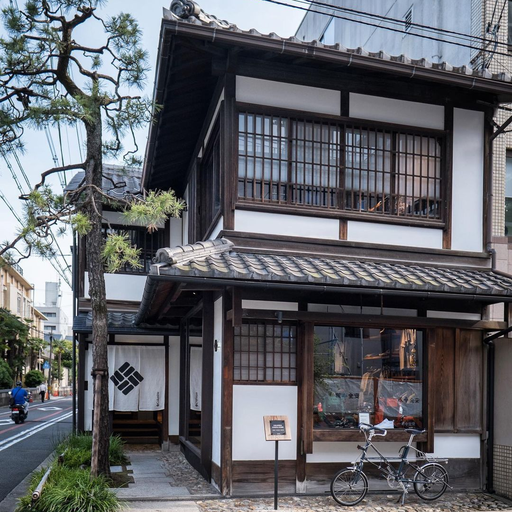
\includegraphics[width=0.47\textwidth]{images/pic1_512x512.png}
    \hfill
    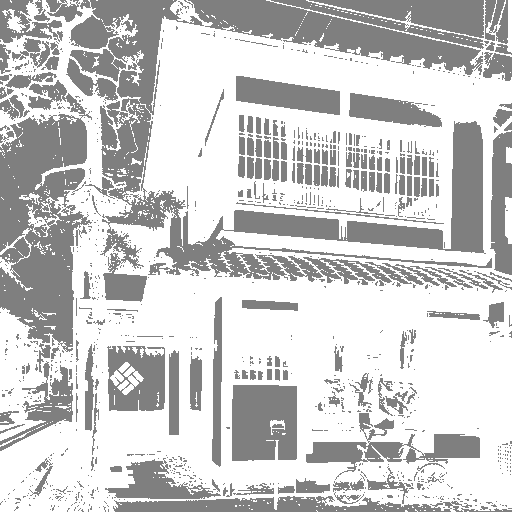
\includegraphics[width=0.47\textwidth]{images/pic1_512x512_classmap.png}
    \caption{Входное изображение и карта классов для кейса 512x512}
\end{figure}

\section*{Выводы}
По полученным замерам видно, что время ядра GPU мало и составляет доли миллисекунды:
для \(512\times512\) примерно \(0.033\mbox{--}0.049\) мс, для \(4096\times4096\)
примерно \(0.725\mbox{--}0.901\) мс. При этом совокупное время GPU заметно больше времени ядра,
так как включает накладные расходы на обмен данными и служебные операции.

На размере \(512\times512\) CPU и GPU дают близкие результаты по полному времени:
CPU \(0.765\) мс, GPU \(0.836\mbox{--}0.858\) мс. На размере \(4096\times4096\)
GPU уже быстрее CPU: CPU \(48.696\) мс против GPU \(29.883\mbox{--}30.271\) мс
(ускорение около \(1.6\\times\)).

По совокупному времени лучшая конфигурация блока в замерах:
\verb|<<<2048, 512>>>| для \(512\times512\) и \verb|<<<32768, 512>>>| для \(4096\times4096\).
Карта классов для изображения \(512\times512\) показывает корректное разделение на два класса,
что подтверждает работоспособность реализации.

\end{document}
